\begin{tikzpicture}
	\tikzstyle{legend}=[rectangle, draw=black, minimum width=1em, minimum height=1em, text width=1em, inner xsep=0]
	\node[anchor=south west,inner sep=0] (image) at (0,0) {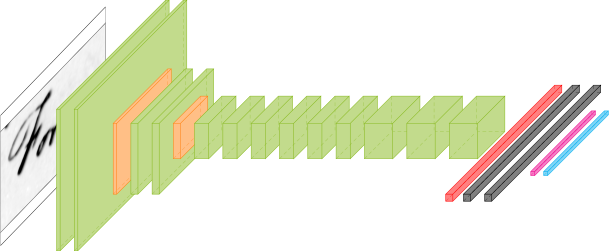
\includegraphics[width=0.9\textwidth]{graphics/phocnet_naked}};
	
	\begin{scope}[x={(image.south east)},y={(image.north west)}]
        %\tikzhelpergrid		        
    			% plot the legend
	\node[legend, fill=tucol2!50, label=right:{\footnotesize{$3\times3$ Convolutional Layer + ReLU}}] at (0.25, 0.1) {};
	\node[legend, fill=tucol1!50, label=right:{\footnotesize{$2\times2$ Max Pooling Layer}}] at (0.25, 0.0) {};
	\node[legend, fill=red!50, label=right:{\footnotesize{$3$-level Spatial Pyramid Max Pooling Layer}}] at (0.25, -0.1) {};
	\node[legend, fill=black!50, label=right:{\footnotesize{Fully Connected Layer + ReLU and Dropout}}] at (0.25, -0.2) {};
	\node[legend, fill=magenta!50, label=right:{\footnotesize{Fully Connected Layer + Linear Activation}}] at (0.25, -0.3) {};
	\node[legend, fill=cyan!50, label=right:{\footnotesize{Sigmoid Activation}}] at (0.25, -0.4) {};
    \end{scope}
\end{tikzpicture}

